% ForceSketch -- NeurIPS 2026 SIMBIOCHEM II workshop submission (non-archival, 5-8pp).
% Swap \documentclass line for the workshop style file when it is available:
%   \usepackage[final]{neurips_2026}
% Every number is drawn from paper/macros.tex, which analysis/tables.py regenerates
% from results/raw/. Do not write a literal result into this file (spec SS68).
\documentclass[10pt]{article}
\usepackage[margin=1in]{geometry}
\usepackage{amsmath,amssymb,booktabs,graphicx,microtype,url}
\usepackage[round]{natbib}
\usepackage[colorlinks,citecolor=blue,linkcolor=blue]{hyperref}
% Generated by analysis/tables.py -- do not edit by hand.
\newcommand{\fsCostIntercept}{10.38}
\newcommand{\fsCostSlope}{11.78}
\newcommand{\fsHaarRecallKTwo}{0.450}
\newcommand{\fsHaarSpearmanKTwo}{0.676}
\newcommand{\fsHaarRecallKThree}{0.529}
\newcommand{\fsHaarSpearmanKThree}{0.781}
\newcommand{\fsHaarRecallKFour}{0.619}
\newcommand{\fsHaarSpearmanKFour}{0.859}
\newcommand{\fsHeadSubRecallKThree}{0.477}
\newcommand{\fsGaussRecallKThree}{0.304}
\newcommand{\fsCeilingKThreeBOne}{1.83}
\newcommand{\fsCeilingKTwoBOne}{2.31}
\newcommand{\fsCeilingKThreeBSixtyFour}{1.87}
\newcommand{\fsCeilingKTwoBSixtyFour}{2.39}
\newcommand{\fsGateSkipThreeBPA}{0.860}
\newcommand{\fsGateRecallThreeBPA}{0.982}
\newcommand{\fsGateSpeedupThreeBPA}{1.25}
\newcommand{\fsGateSkipEthanol}{0.793}
\newcommand{\fsGateRecallEthanol}{0.973}
\newcommand{\fsGateSpeedupEthanol}{1.16}
\newcommand{\fsGateSkipAspirin}{0.765}
\newcommand{\fsGateRecallAspirin}{0.988}
\newcommand{\fsGateSpeedupAspirin}{1.12}
\newcommand{\fsGateSkipAzobenzene}{0.849}
\newcommand{\fsGateRecallAzobenzene}{0.971}
\newcommand{\fsGateSpeedupAzobenzene}{1.23}
\newcommand{\fsStableRank}{5.13}
\newcommand{\fsTopEigFraction}{0.334}


\title{ForceSketch: Randomized Head-Space VJPs for Screening\\Force Uncertainty in Multi-Head Molecular Potentials}
% SIMBIOCHEM II is DOUBLE-BLIND: non-anonymized submissions are desk-rejected.
% Do not restore an author block before checking the venue's policy.
\author{Anonymous submission}
\hypersetup{pdfauthor={},pdftitle={},pdfsubject={},pdfkeywords={}}
\date{}

\begin{document}
\maketitle

\begin{abstract}
Multi-head committees make ensemble \emph{energy} uncertainty nearly free for machine-learned
interatomic potentials: one forward pass yields all $M$ head energies. Force uncertainty is not,
since a single backward pass cannot produce the per-head forces --- exact disagreement needs the
full $(M{-}1)$-dimensional centered head subspace. We ask whether $K\ll M{-}1$ randomized or
orthogonal head-space vector--Jacobian products can stand in, using unbiased Gaussian and Haar
estimators with exact finite-$K$ corrections, on a pretrained eight-head MACE committee across 3BPA
and three rMD17 molecules. The answer is negative for \emph{replacement} and positive for
\emph{screening}. At $K\le4$ no estimator recovers the exact top-5\% uncertainty set (best
\fsHaarRecallKFour{} \fsHaarRecallKFourCI{}). But a conservatively calibrated gate over a low-rank
head-space control variate skips
\fsGateSkipThreeBPA{} of exact evaluations while retaining \fsGateRecallThreeBPA{} of
high-uncertainty configurations, on all four systems. The wall-clock benefit is sharply
regime-dependent: against a \emph{batched} exact baseline, reducing directions is worth
$\fsBestTotalKThreeBSixteen\times$ at batch size 16 but only $\fsBestTotalKThreeBOne\times$ at batch
size 1, where batched reverse mode already amortizes cotangent lanes and the gate becomes a net
slowdown. The decision-quality result is robust; the speed result is not.
\end{abstract}

\section{Introduction}
Uncertainty quantification is what makes learned interatomic potentials usable beyond their training
distribution: it drives active learning, flags extrapolation during molecular dynamics, and decides
when a reference calculation is required. Committee disagreement remains the most widely used
estimator, and multi-head committees~\citep{beck2025mhc} make it dramatically cheaper by attaching
$M$ readout heads to one shared message-passing trunk, so that all $M$ energies come from a single
forward pass.

That amortization does not extend to forces. As the multi-head committee work states directly,
``a single backward pass can not yield the forces for all the heads, and thus their standard
deviation \ldots\ the standard deviation requires multiple reverse passes through the computational
graph.'' Forces are the quantity that matters for MD and for most acquisition rules, so the
expensive half of committee UQ is exactly the half the shared trunk fails to amortize.

Downstream, however, one rarely needs every member force. Acquisition needs a \emph{ranking};
a safety gate needs a \emph{threshold decision}; error analysis needs the most uncertain
\emph{atom}. This motivates estimating the force-variance statistic directly rather than
reconstructing the member forces that define it. We call this ForceSketch: replace the exact
$(M{-}1)$-direction centered head basis with $K$ randomized or orthogonal head-space directions,
each costing one reverse pass.

\paragraph{Contributions.}
First, we formulate multi-head force disagreement as a statistic of the centered energy Jacobian
with respect to atomic coordinates, and show the exact computation needs only the centered
$(M{-}1)$-dimensional head subspace. Second, we give unbiased Gaussian, Haar-orthogonal,
Rademacher and pairwise estimators, with closed-form finite-$K$ corrections for the componentwise
force standard deviation; we correct a removable singularity in the Haar constant and verify every
estimator by Monte Carlo. Third, we report a \emph{negative} result that we believe is the useful
one: at $K\le4$ none of these estimators preserves the exact top-5\% acquisition set, on any of four
molecular systems. Fourth, we show what does work --- a conservatively calibrated screening gate
with a low-rank control variate --- and quantify both its decision quality and its wall-clock saving.

\begin{figure}[t]
\centering
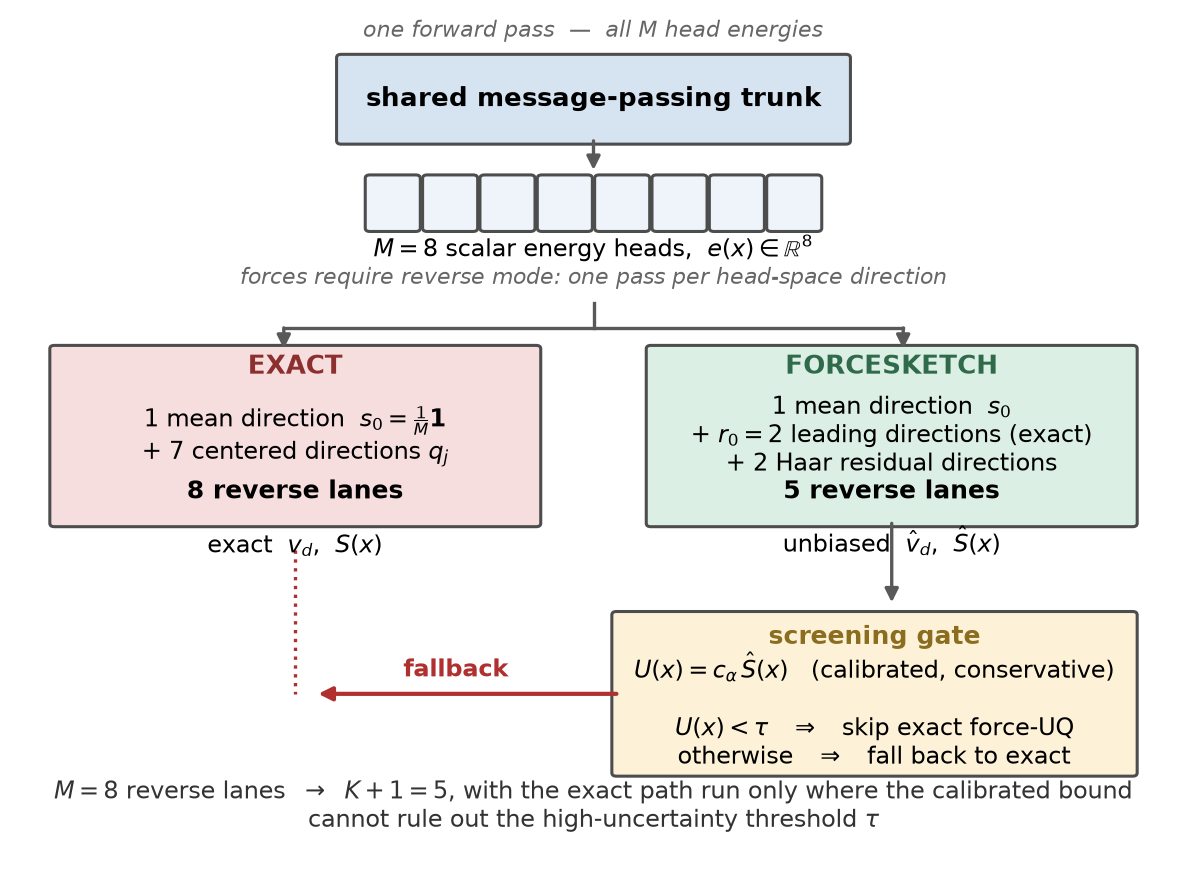
\includegraphics[width=0.86\textwidth]{figures/fig1_schematic.png}
\caption{What ForceSketch replaces. All $M$ head energies come from one forward pass through the
shared trunk, but forces do not: each head-space direction costs its own reverse pass, so exact
force disagreement needs $M$ lanes. ForceSketch spends $K{+}1$, and --- since the approximation is
not accurate enough to \emph{replace} exact uncertainty at $K\le4$ (Section~\ref{sec:fidelity}) --- its score
feeds a conservatively calibrated gate that runs the exact path only where the bound cannot rule
out the high-uncertainty threshold.}
\label{fig:schematic}
\end{figure}

\section{Problem formulation}
For Cartesian coordinates $x\in\mathbb{R}^{D}$, $D=3N$, a multi-head committee defines energies
$e(x)=[E_1(x),\dots,E_M(x)]^{\mathsf T}$ and head forces $f_m=-\nabla_x E_m$, collected as
$F(x)\in\mathbb{R}^{D\times M}$. With the centering projector $P = I - \tfrac{1}{M}\mathbf{1}\mathbf{1}^{\mathsf T}$,
the per-coordinate disagreement is
\begin{equation}
v_d \;=\; \frac{1}{M-1}\sum_{m}\bigl(F_{dm}-\bar F_d\bigr)^2 \;=\; \frac{1}{M-1}\bigl\|e_d^{\mathsf T}FP\bigr\|_2^2 ,
\qquad S \;=\; \sum_d v_d \;=\; \frac{\|FP\|_F^2}{M-1},
\end{equation}
with atom-level scores $u_a^{\mathrm{RMS}}=\sqrt{\tfrac13\sum_\alpha v_{a\alpha}}$ and
$u_a^{\mathrm{MHC}}=\tfrac13\sum_\alpha\sqrt{v_{a\alpha}}$.

Let $Q\in\mathbb{R}^{M\times(M-1)}$ satisfy $Q^{\mathsf T}Q=I$, $Q^{\mathsf T}\mathbf 1=0$,
$QQ^{\mathsf T}=P$. Each column gives one reverse pass, $g_j=-\nabla_x(q_j^{\mathsf T}e)=Fq_j$, and
$v_d=\tfrac{1}{M-1}\sum_j g_{j,d}^2$. The mean force is one further seed, $s_0=\tfrac1M\mathbf 1$.
Exact force UQ therefore costs $M$ reverse lanes in total. \emph{Our question is whether downstream
uncertainty decisions require all $M-1$ centered directions.}

\section{Method}
\paragraph{Gaussian and Haar sketches.}
Draw $z_k\sim\mathcal N(0,I_M)$ and center, $w_k=Pz_k$; one reverse pass gives $g_k=Fw_k$ and
$\widehat v_d = \tfrac{1}{K(M-1)}\sum_k g_{k,d}^2$ is unbiased. Alternatively sample a Haar-random
orthonormal $K$-frame $W=QO$ inside the centered space; then
$\widehat v^{\mathrm{Haar}}_d = \tfrac1K\sum_k G_{dk}^2$ is unbiased and \emph{exact} at $K=M-1$.
Writing $r=M-1$, the two have relative standard deviations $\sqrt{2/K}$ and
$\sqrt{2(r-K)/(K(r+2))}$, so orthogonalization reduces estimator variance by exactly
$(r-K)/(r+2)$ --- a factor of $4/9$ at $K{=}3$, $M{=}8$. This is free, and it is the single largest
methodological lever we find.

\paragraph{Finite-$K$ corrections.}
$\sqrt{\widehat v_d}$ is biased low. For Gaussian probes $K\widehat v_d/v_d\sim\chi^2_K$ and the
correction is $c_K=\sqrt{2/K}\,\Gamma(\tfrac{K+1}{2})/\Gamma(\tfrac K2)$. For Haar probes the
analogous constant is conventionally written with Beta functions, which is singular at $K=r$
(it evaluates $B(K/2,0)$). Cancelling the shared $\Gamma(\tfrac{r-K}{2})$ gives a form that is
finite everywhere and exactly $1$ at full rank:
\begin{equation}
c^{\mathrm{Haar}}_{K,r}\;=\;\sqrt{\tfrac{r}{K}}\;
\frac{\Gamma\!\left(\tfrac{K+1}{2}\right)\Gamma\!\left(\tfrac r2\right)}
     {\Gamma\!\left(\tfrac K2\right)\Gamma\!\left(\tfrac{r+1}{2}\right)} ,
\qquad c^{\mathrm{Haar}}_{K,r}\to c_K \ \text{ as } r\to\infty .
\end{equation}
We verify unbiasedness of $\sqrt{\widehat v}/c$ to within Monte-Carlo error at $4\times10^5$ draws.

\paragraph{Low-rank control variate.}
Split $P = Q_{r_0}Q_{r_0}^{\mathsf T} + R$, where $Q_{r_0}$ holds the $r_0$ leading eigenvectors of
the calibration-set average $\bar A=\tfrac1n\sum_i PF_i^{\mathsf T}F_iP$. Evaluate those $r_0$
directions exactly and sketch only the residual with $K'=K-r_0$ Haar directions:
\begin{equation}
\widehat v_d \;=\; \frac{1}{r}\Bigl[\textstyle\sum_{j\le r_0} g_{j,d}^2 \;+\; \frac{r-r_0}{K'}\sum_{k} G_{k,d}^2\Bigr],
\end{equation}
which remains unbiased. We stress the motivation is the \emph{opposite} of the intuitive one: a
concentrated spectrum does not explain why small $K$ works, it is what \emph{breaks} a random sketch,
because the sketch either captures the dominant directions or misses them.

\paragraph{Screening rather than replacement.}
Given a cheap $\widehat S$, calibrate $c_\alpha$ as the $(1-\alpha)$ quantile of
$S(x_i)/\widehat S(x_i)$ on a held-out calibration split and define the optimistic bound
$U(x)=c_\alpha\widehat S(x)$. For an exact high-uncertainty threshold $\tau$, skip the exact
computation when $U(x)<\tau$ and fall back otherwise. The gate is conservative by construction:
$U$ over-estimates $S$ for $(1-\alpha)$ of calibration structures.

\section{Experimental setup}
We use the pretrained eight-head MACE committees released with~\citep{beck2025mhc}: two message-passing
layers, 32 channels, $\ell_{\max}=1$, $r_{\mathrm{cut}}=6$\,\AA. We evaluate the three
head-distribution variants (\emph{disjoint}, \emph{overlapping}, \emph{same}) on 3BPA at 1200\,K
(2139 structures, extrapolative relative to the 300\,K training set) and the joint ten-molecule
rMD17 committee on ethanol (9 atoms), aspirin (21) and azobenzene (24), 1000 held-out structures each.
All estimator evaluation is in float64. This is not fastidiousness: with mean force over disagreement
$\rho\approx36$ on this committee, a float32 ``exact'' reference carries $\sim\!3\times10^{-5}$
relative error, larger than the $10^{-5}$ tolerance at which we verify full-rank exactness.
Ten random seeds are frozen before testing and none is discarded; all confidence
intervals are paired bootstraps over structures with \fsNBoot{} resamples. Timing uses CUDA events with
per-iteration measurement on an RTX 5070 Laptop GPU; the measured lane cost is
$T(L)=\fsCostIntercept + \fsCostSlope\,L$\,ms.

\section{Results}

\subsection{Can force disagreement be sketched?}
\label{sec:fidelity}
Figure~\ref{fig:pareto} gives the answer: partially, and not well enough to replace exact
computation. Haar is the best sketch at every budget --- top-5\% recall \fsHaarRecallKTwo,
\fsHaarRecallKThree{} \fsHaarRecallKThreeCI{} and \fsHaarRecallKFour{} \fsHaarRecallKFourCI{} at
$K=2,3,4$. Rank correlation is respectable (Spearman \fsHaarSpearmanKFour{}
\fsHaarSpearmanKFourCI{} at $K{=}4$), but tail selection is not: no method approaches the 0.90
recall that would justify substitution. All intervals are 95\% paired bootstrap over structures
(\fsNBoot{} resamples), computed on the seed-averaged statistic; seed-to-seed standard deviations are
$0.03$--$0.06$ and are reported separately in the result records.

Orthogonalizing the probes is the largest single lever in the method. The paired difference between
Haar and Gaussian at $K{=}3$, evaluated on identical structure resamples, is
$\fsDeltaOrtho$ \fsDeltaOrthoCI{} in top-5\% recall, and is significant on all four systems. The
low-rank control variate adds a further $\fsDeltaCV$ \fsDeltaCVCI{} over Haar at $K{=}4$, reaching
\fsCVRecallKFour{} \fsCVRecallKFourCI{} --- still short of 0.90.

The head-space spectrum explains why. Writing $A=\bar{Q^{\mathsf T}F^{\mathsf T}FQ}$ for the averaged
centered force-disagreement Gram matrix, the stable rank of the matrix we actually sketch is
$\operatorname{srank}(FQ)=\|FQ\|_F^2/\|FQ\|_2^2=\operatorname{tr}(A)/\lambda_{\max}
=\fsSrankLo$--$\fsSrankHi$ of a maximum $7$ across the four systems, with the leading direction
carrying $\fsTopEigLo$--$\fsTopEigHi$ of the disagreement (an isotropic spectrum would give
$\fsTopEigIsotropic$). The spectrum is therefore \emph{moderately diffuse rather than strongly
rank-concentrated} --- but far from isotropic, at roughly $2.3\times$ the isotropic leading share.
That is exactly the regime in which a random $K$-dimensional projection pays a variance penalty, and
it is why projecting out the leading directions (the control variate) recovers so much.

\begin{figure}[t]
\centering
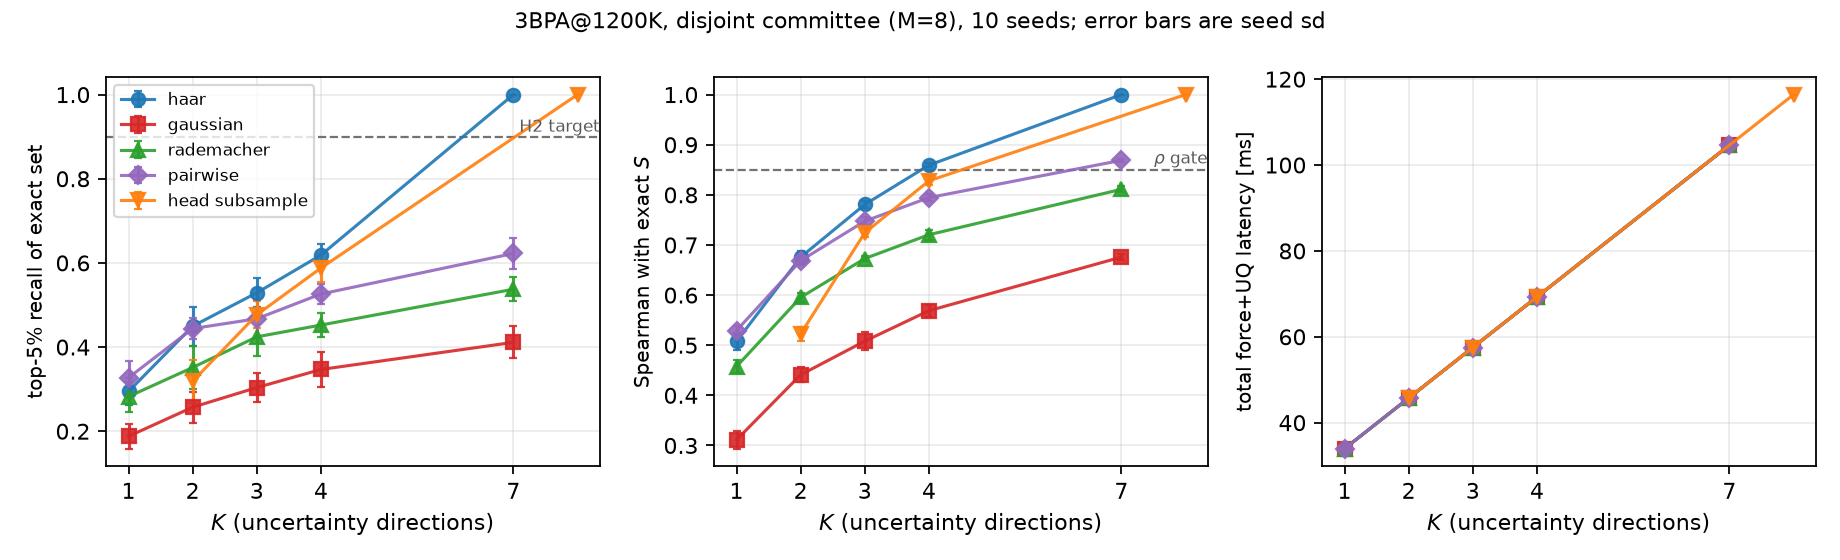
\includegraphics[width=\textwidth]{figures/fig3_k_tradeoff.png}
\caption{Accuracy and cost against $K$. The latency curves coincide exactly for every method,
because cost depends only on the lane count --- so the two accuracy panels are the whole trade-off.
Ranking saturates well before tail selection does: Haar clears $\rho=0.85$ at $K{=}4$ while its
top-5\% recall is still $\fsHaarRecallKFour$. Error bars are the standard deviation across the ten
frozen seeds.}
\label{fig:ktradeoff}
\end{figure}

\subsection{Does sketching beat using fewer heads?}
It depends on whether an exact mean force is required, and the two framings give opposite answers,
so we report both. At equal total reverse lanes \emph{with} an exact mean force, Haar at $K{=}3$
beats head subsampling at $K{=}3$ plus a mean lane by $\fsDeltaVsHeadSub$ \fsDeltaVsHeadSubCI{} in
top-5\% recall (paired bootstrap on identical resamples). That ordering is significant on 3BPA,
ethanol and azobenzene, and consistent in sign but \emph{not} significant on aspirin
($+0.030$, CI $[-0.022, 0.070]$). Conversely, head subsampling at $K{=}4$ with no mean lane spends the
same four lanes and scores significantly \emph{higher} ($-0.059$, CI $[-0.094,-0.023]$ for Haar) ---
but it cannot produce the mean force molecular dynamics requires. Reporting a single framing would
have settled this comparison by definition rather than by measurement.

\subsection{Does reducing directions reduce GPU time?}
\label{sec:regime}
Only in some regimes, and the honest answer required first making the strongest baseline available.

\paragraph{Batched reverse mode, and why it initially appeared impossible.}
\texttt{torch.autograd.grad(is\_grads\_batched=True)} vectorizes the backward over cotangents while
reusing one forward graph, and is the baseline spec-level fairness demands. On this stack it fails
with \texttt{Cannot access data pointer of Tensor that doesn't have storage} --- but only from the
third call onwards, which disguises the cause. The mechanism is: batched reverse mode runs under
\texttt{torch.\_vmap\_internals}, so cotangents are \texttt{BatchedTensor}s with no storage;
TorchScript's profiling executor emits an optimized plan only after two warm-ups; and the TensorExpr
fuser then fuses the \emph{reverse} graph into a \texttt{prim::TensorExprGroup}, whose kernel
requires a raw \texttt{data\_ptr()} for every input. The TorchScript on the path is
\texttt{e3nn}'s \texttt{\_spherical\_harmonics}, a module-level \texttt{@torch.jit.script}
\emph{free function} --- not a module, so walking the module tree finds nothing to un-script, and a
fully rebuilt zero-\texttt{ScriptModule} model still fails. Disabling the TensorExpr fuser before
the first forward fixes it: 50/50 consecutive batched calls agreeing with the serial path to
$3\times10^{-15}$, at a $\sim\!4\%$ cost to the serial path from losing fusion. We report this
because it is a trap any e3nn-based UQ work will hit, and because without it we would have compared
against a Python loop, which spec-level fairness forbids.

\paragraph{Two speedups, never conflated.}
We report both quantities the protocol distinguishes, since they answer different questions. With
$T(L)$ the latency of an $L$-lane reverse pass, $M$ the committee size and $K$ the sketch budget,
\begin{equation}
\text{incremental UQ}=\frac{T(M)-T(1)}{T(1{+}K)-T(1)},
\qquad
\text{total force+UQ}=\frac{T(M)}{T(1{+}K)} ,
\end{equation}
the first being the cost of uncertainty once the mean force is paid for, the second including it.
Every figure below states which one it plots, at which batch size, against which implementation.
Note the incremental ratio is unstable at small batch precisely because $T(1{+}K)\approx T(1)$ there,
which is the effect this section is about; we therefore lead with the total.

\paragraph{With that baseline, the benefit is regime-dependent.}
Batched reverse mode is dramatically better at small batch: at $B{=}1$ it takes
$\fsBatchedFlatLaneOne$\,ms for one lane and $\fsBatchedFlatLaneEight$\,ms for eight --- nearly
\emph{flat} in the lane count, so additional cotangents are almost free. ForceSketch's total
force-plus-UQ speedup at $K{=}3$ therefore collapses to $\fsBestTotalKThreeBOne\times$ at $B{=}1$,
against $1.83\times$ if one compares only to a serial loop. At $B{=}16$ the batched path scales with
$L$ again and the speedup recovers to $\fsBestTotalKThreeBSixteen\times$; at $B{=}64$ the batched
path exhausts the 8\,GB card and the serial loop wins, giving $1.86\times$. Incremental UQ speedups
are $\fsBestIncrKThreeBOne\times$ and $\fsBestIncrKThreeBSixteen\times$ at $B{=}1$ and $B{=}16$,
but that statistic is unstable at small batch precisely because $T(L{=}1{+}K)\approx T(L{=}1)$ there.

\begin{center}\small
\begin{tabular}{lrrrr}
\toprule
 & \multicolumn{2}{c}{$B=1$ (27 atoms)} & \multicolumn{2}{c}{$B=16$ (432 atoms)} \\
lanes $L$ & serial & batched & serial & batched \\
\midrule
1 & 22.9 & 25.5 & 24.3 & 26.0 \\
4 & 60.3 & \textbf{27.5} & 62.5 & \textbf{39.7} \\
8 & 110.5 & \textbf{30.5} & 115.6 & \textbf{73.2} \\
\bottomrule
\end{tabular}
\end{center}

A kernel-level profile of the serial path explains why removing lanes helps at all when it does: the
composition of GPU time is invariant in $L$ (elementwise $42.2\%$ at $L{=}7$ against
$41.5$--$41.9\%$ at $L{=}2,3,4$; tensor products $21.3\%$ against $20.0$--$20.9\%$; the same $134$
distinct kernels throughout), and only the repetition count changes --- $10{,}161$ launches per exact
step against $4{,}796$ at $K{=}3$. Sketching linearly reduces repeated execution of the shared
trunk. Batched reverse mode attacks the same redundancy by a different route, which is exactly why
the two are substitutive at small batch.

\paragraph{Partial compilation.}
For completeness we also compiled the model. \texttt{torch.compile} succeeds only partially here ---
Dynamo builds a sequence-length guard on e3nn's \texttt{Irrep} and calls \texttt{len()} on it, which
e3nn raises \texttt{NotImplementedError} for by design, so untraceable regions must fall back to
eager. With that, compilation is correct to $\fsCompileRelErr$ and gives
$\fsCompileSpeedupLo$--$\fsCompileSpeedupHi\times$ at $B{=}16$. The absolute saving grows linearly in
$L$, so AOTAutograd is producing a cheaper backward rather than merely a faster forward. We report
the eager batched path as primary because it is portable and needs no fallback workaround, and note
that compilation would shift the numbers here by at most a few percent in the same direction for
every method, leaving the crossover of Section~\ref{sec:regime} unchanged.

\subsection{Can approximate screening avoid exact computation?}
This is where the method succeeds. With a control variate at $r_0{=}2$, $K{=}4$ and $\alpha{=}0.05$,
evaluated on held-out test splits with $c_\alpha$ and $\tau$ fitted only on calibration data:

\begin{center}\small
\begin{tabular}{lrrrr}
\toprule
system & high-UQ recall & exact skipped & screening speedup \\
\midrule
3BPA @ 1200\,K   & \fsGateRecallThreeBPA   & \fsGateSkipThreeBPA   & $\fsGateSpeedupThreeBPA\times$ \\
rMD17 ethanol    & \fsGateRecallEthanol    & \fsGateSkipEthanol    & $\fsGateSpeedupEthanol\times$ \\
rMD17 aspirin    & \fsGateRecallAspirin    & \fsGateSkipAspirin    & $\fsGateSpeedupAspirin\times$ \\
rMD17 azobenzene & \fsGateRecallAzobenzene & \fsGateSkipAzobenzene & $\fsGateSpeedupAzobenzene\times$ \\
\bottomrule
\end{tabular}
\end{center}

Roughly four in five exact force-UQ evaluations are avoided while $97\%$--$99\%$ of
high-uncertainty configurations are still routed to the exact computation. These are properties of
the estimator and are unaffected by the choice of exact implementation.

The wall-clock saving is a different matter, and inherits the regime dependence of Section~\ref{sec:regime}. The
gate pays $K{+}1$ lanes on \emph{every} structure and $M$ lanes on the minority it cannot clear, so
it only pays off when lanes are expensive. Against the strongest exact baseline it is
$\fsBestGateSpeedupBSixteen\times$ at $B{=}16$ and $1.26\times$ at $B{=}64$, but
$\fsBestGateSpeedupBOne\times$ at $B{=}1$ --- a net \emph{slowdown}, because batched reverse mode
makes eight lanes nearly as cheap as five. The gate is therefore worth running for batched
active-learning sweeps and not for single-structure MD steps, and we would rather say so than quote
the serial-baseline figure of $1.23\times$.

\begin{figure}[t]
\centering
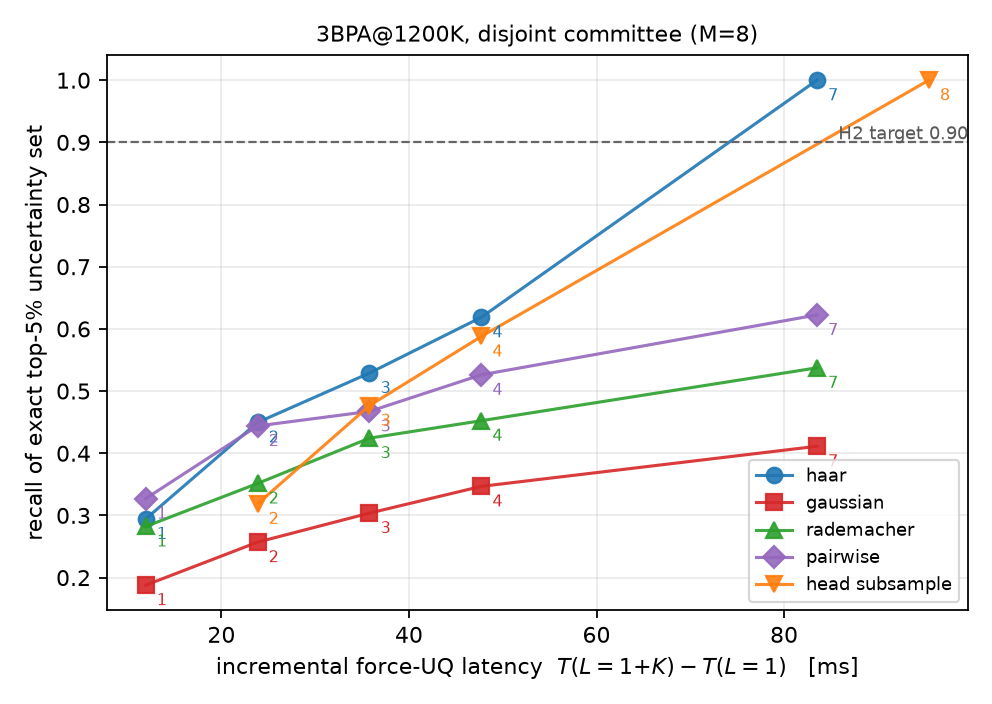
\includegraphics[width=0.49\textwidth]{figures/fig2_pareto_disjoint_test_1200K.png}
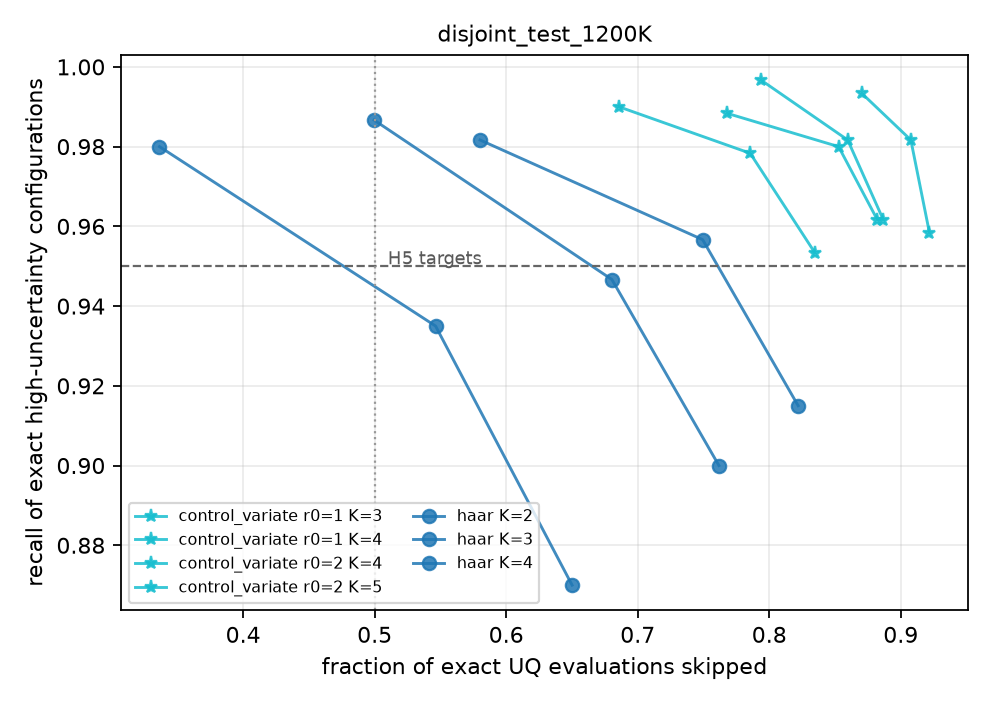
\includegraphics[width=0.49\textwidth]{figures/fig5_screening_disjoint_test_1200K.png}
\caption{Left: accuracy--latency Pareto on 3BPA@1200\,K; no method reaches the 0.90 recall line
before the exact budget. Right: the screening gate --- fraction of exact evaluations skipped against
retained high-uncertainty recall.}
\label{fig:pareto}
\end{figure}

\section{Limitations}
\label{sec:limitations}
\textbf{The systems benefit is regime-dependent, and absent at $B{=}1$.} With batched reverse mode
enabled, extra cotangent lanes are nearly free at small batch, so ForceSketch's total speedup falls
to $\fsBestTotalKThreeBOne\times$ and the screening gate becomes a net slowdown
($\fsBestGateSpeedupBOne\times$). Single-structure MD --- the deployment regime that matters most ---
is precisely where this method does not pay for itself on this hardware. \textbf{Lane memory.}
Batched reverse mode holds $L$ cotangent sets at once and exhausts an 8\,GB card at $B{=}64$, where
the serial loop wins; that crossover will sit elsewhere on a larger accelerator, and we have only one
GPU. \textbf{\texttt{torch.func} is unavailable}: MACE calls \texttt{requires\_grad\_()} inside
\texttt{forward}, which functorch forbids, and a globally installed no-op shim silently returns
all-zero gradients rather than raising --- a trap worth naming.
\textbf{Other limitations:} the estimator is approximate for $K<M-1$ and, on these systems, not
accurate enough to replace exact UQ; extreme-value statistics (most-uncertain atom) converge more
slowly than global ones; committee disagreement is only a proxy for error; calibration may shift
out of distribution; $M{=}8$ bounds the maximum possible saving; rMD17 spans only 9--24 atoms, so
molecule size is a weak axis; and cuEquivariance is unavailable for this readout, so all baselines
are e3nn-only.

\section{Conclusion}
Exact multi-head force uncertainty cannot be replaced by a handful of randomized head-space VJPs at
the fidelity acquisition requires: we could not reach 0.90 top-5\% recall below $K\approx6$ of $7$
on any of four systems. The head-space spectrum is moderately concentrated
($\operatorname{srank}(FQ)=\fsSrankLo$--$\fsSrankHi$ of $7$), which is both why an oblivious random
sketch pays a variance penalty and why projecting out the leading directions recovers part of it.

It can, however, be \emph{screened}. A conservatively calibrated gate over a control-variate sketch
avoids roughly four in five exact force-UQ computations while retaining $97$--$99\%$ of
high-uncertainty structures, on every system tested. That decision-quality result is a property of
the estimator and holds regardless of implementation.

Whether it saves time is a separate question, and the honest answer is: only in batch. Once batched
reverse mode is enabled --- which on this stack required disabling the TensorExpr fuser, since e3nn's
scripted spherical harmonics otherwise fuse the reverse graph into a kernel that cannot accept
batched cotangents --- extra cotangent lanes become nearly free at $B{=}1$, and both the sketch and
the gate stop paying for themselves. The method is therefore worth deploying for batched
active-learning sweeps over candidate structures, and not for single-structure MD steps. We think
the more useful contribution is the measurement that separates those two regimes, together with the
observation that orthogonalizing the probes is free and worth more than any other single choice in
the estimator design.

\bibliographystyle{plainnat}
\begin{thebibliography}{9}
\bibitem[Beck et al.(2025)]{beck2025mhc} H.~Beck, P.~Simko, L.~L.~Schaaf, O.~Marsalek, and C.~Schran.
Multi-head committees enable direct uncertainty prediction for atomistic foundation models.
\emph{J. Chem. Phys.} 163, 234103 (2025). arXiv:2508.09907.
\bibitem[Batatia et al.(2022)]{mace} I.~Batatia, D.~P.~Kov\'acs, G.~N.~C.~Simm, C.~Ortner, and G.~Cs\'anyi.
MACE: Higher order equivariant message passing neural networks for fast and accurate force fields.
\emph{NeurIPS} (2022).
\bibitem[Kov\'acs et al.(2021)]{botnet} D.~P.~Kov\'acs et al. Linear atomic cluster expansion force fields
for organic molecules. \emph{J. Chem. Theory Comput.} 17, 7696 (2021). [3BPA dataset]
\bibitem[Christensen \& von Lilienfeld(2020)]{rmd17} A.~S.~Christensen and O.~A.~von Lilienfeld.
On the role of gradients for machine learning of molecular energies and forces.
\emph{Mach. Learn.: Sci. Technol.} 1, 045018 (2020). [rMD17]
\bibitem[Hutchinson(1990)]{hutchinson} M.~F.~Hutchinson. A stochastic estimator of the trace of the
influence matrix for Laplacian smoothing splines. \emph{Commun. Stat. Simul. Comput.} 19, 433 (1990).
\end{thebibliography}

\end{document}
